\documentclass[11pt]{article}
\usepackage[margin=0.82in]{geometry}
\usepackage[T1]{fontenc}
\usepackage{lmodern}
\usepackage{microtype}
\usepackage{amsmath,amssymb,mathtools}
\usepackage{graphicx}
\usepackage{booktabs,tabularx,array,longtable}
\usepackage{enumitem}
\usepackage{xcolor}
\usepackage{caption}
\usepackage[numbers,sort&compress]{natbib}
\usepackage{hyperref}
\usepackage{float}
\hypersetup{colorlinks=true,linkcolor=blue!45!black,citecolor=blue!45!black,urlcolor=blue!45!black,
 pdftitle={Beyond the Biological Bottleneck: Can Intelligence Emerge Directly from Nature?},
 pdfauthor={Devanik Debnath},pdfsubject={Abiotic intelligence, natural computation, astrobiology and SETI}}
\graphicspath{{figures/}}
\setlength{\parskip}{0.38em}
\setlength{\parindent}{0pt}
\setlist{itemsep=0.12em,topsep=0.25em,leftmargin=1.4em}
\captionsetup{font=small,labelfont=bf}
\newcommand{\HD}{H_{\mathrm{D}}}
\newcommand{\HC}{H_{\mathrm{C}}}
\newcommand{\HN}{H_{\mathrm{N}}}
\newcommand{\KL}{D_{\mathrm{KL}}}
\newcommand{\doop}{\operatorname{do}}
\newcommand{\E}{\mathbb{E}}
\newcommand{\MI}{\mathsf{I}}

\title{\vspace{-1.15em}\textbf{Beyond the Biological Bottleneck: Can Intelligence Emerge Directly from Nature?}\\[0.35em]
\large A Framework for Natural Computation, Abiotic Agency, and Distinguishing Emergence from Construction}
\author{Devanik Debnath\\\small Independent research preprint\\\small \href{https://github.com/Devanik21}{GitHub: Devanik21}}
\date{30 October 2026}

\begin{document}
\maketitle

\begin{abstract}
On Earth, the familiar historical route to artificial intelligence passes through biological evolution: physical and chemical processes gave rise to life, biological evolution produced intelligence, and intelligent organisms engineered non-biological computing systems. This sequence is an observation about one planet, not an established universal law. Could a non-living physical system develop persistent information processing, adaptive learning, prediction, and goal-directed control without a biological evolutionary stage? Recent work makes the question more precise: a self-organising formose reaction network has been demonstrated to perform nonlinear classification and time-series forecasting, while physical reservoir computing provides a general framework for exploiting material dynamics as computational substrates. Neither result demonstrates autonomous agency or intelligence. We therefore separate physical computation, adaptive computation, minimal agency, biological status, and causal origin. We define three origin hypotheses: direct abiotic emergence, intelligence-mediated construction, and a non-intelligent natural decoy. A central identifiability result follows: if direct-emergence and construction hypotheses induce the same distribution over functional observations, no classifier using those observations alone can infer origin better than the prior odds. A reproducible synthetic demonstration illustrates this point: under deliberately matched functional distributions, origin classification is at chance using function alone, while an assumed provenance channel improves classification in the toy model. This is not an empirical estimate of extraterrestrial detectability. We propose a staged observation framework combining intervention-based capability tests, information-theoretic and thermodynamic measurements, provenance evidence, environmental context, and temporal history. The framework is intended to generate falsifiable experiments and disciplined search strategies, not to claim that abiotic intelligence exists. Its central conclusion is methodological: the emergence of non-biological intelligence and the origin of that intelligence are separate scientific questions, and evidence for one does not automatically settle the other.
\end{abstract}

\textbf{Keywords:} astrobiology; abiotic intelligence; natural computation; physical reservoir computing; chemical computation; causal emergence; thermodynamics of computation; technosignatures; SETI; Bayesian model comparison

\section{Introduction: the biological bottleneck}

The human story suggests a simple sequence. Matter formed stars and planets; planetary chemistry enabled prebiotic evolution; life emerged; biological evolution produced nervous systems and human intelligence; and human intelligence constructed artificial computation. This pathway can be written schematically as
\begin{equation}
  \text{natural processes}\;\longrightarrow\;\text{life}\;\longrightarrow\;
  \text{biological intelligence}\;\longrightarrow\;\text{engineered AI}.
  \label{eq:earthpath}
\end{equation}
The sequence is historically familiar, but it does not establish that biological evolution is a necessary intermediate for every possible form of intelligence. Earth provides one realised pathway, not a sample large enough to infer a universal requirement.

The motivating question is therefore not whether today's computers are intelligent, nor whether a mineral, plasma filament, or chemical oscillator should be called alive. It is narrower and more testable: \emph{can non-living physical matter, without an antecedent biological lineage or an intelligence-mediated design process, develop systems with operationally measurable capacities for computation, memory, adaptive learning, prediction, and control?} If such a system were observed elsewhere, a second question would immediately follow: did it emerge through natural processes, or was it built by another intelligence?

This question sits at the intersection of astrobiology, origins-of-life research, nonlinear dynamics, information theory, physical computing, statistical mechanics, and the search for extraterrestrial intelligence (SETI). The intersections matter because each field supplies a different piece of the problem. Chemical reaction networks can compute; autocatalytic organisation helps describe prebiotic chemical closure; physical reservoir computing clarifies when a material substrate implements an input-output computation; information thermodynamics constrains the physical costs of memory and computation; and technosignature research supplies methods for evaluating possible technological artefacts. None alone answers whether intelligence can emerge abiotically.

We make four contributions. First, we separate five concepts that are often conflated: physical dynamics, computation, adaptive computation, agency, and intelligence. Second, we distinguish substrate from origin: a non-biological system may be naturally emergent, constructed, or of unresolved provenance. Third, we formulate an identifiability result showing why functional behaviour alone may be insufficient to distinguish natural emergence from construction. Fourth, we provide a synthetic, reproducible illustration and a staged research programme for laboratory analogues and future astronomical or planetary observations.

The scope is deliberately conservative. We do not claim a discovered abiotic intelligence, a universal definition of intelligence, or a systematic review of every related field. The literature search was targeted to foundational and directly adjacent work available by 30 October 2026. The proposed signatures and tests are research hypotheses requiring independent experimental calibration.

\section{Conceptual boundaries: what is being detected?}

\subsection{Non-biological is not synonymous with abiotic}

A crucial distinction is between the material substrate of a system and the process that produced it. A system need not use terrestrial DNA, proteins, or cells to be a living system in a broader functional sense. Conversely, a system can be made of familiar inorganic matter and still be an artefact constructed by an intelligent agent. We therefore use the terms as follows:
\begin{itemize}
  \item \textbf{Non-biological substrate} means that the operative system is not implemented by an Earth-like biological organism or its familiar molecular machinery. It is a statement about implementation, not ancestry.
  \item \textbf{Abiotic emergence} means that the organisation and adaptive capacities arise through natural physical and chemical processes without a biological evolutionary lineage being the causal source and without an antecedent intelligence deliberately constructing the system.
  \item \textbf{Intelligence-mediated construction} means that an earlier intelligent system deliberately designed, assembled, or substantially organised the observed system. The constructor could itself be biological or non-biological.
  \item \textbf{Biological evolution} means a lineage-level process involving heredity with variation and differential persistence or reproduction. The exact boundary of life remains contested; this operational use is not intended as a universal definition.
\end{itemize}

A non-carbon organism that reproduces and evolves could be biologically organised in this functional sense even if its chemistry is unfamiliar. It should not be counted as abiotic merely because an Earth-centred biochemical assay fails. This caution parallels current work on agnostic biosignatures, which seeks functional and contextual criteria rather than assuming molecular similarity to Earth life \citep{Graham2026,Barge2026}. The word \emph{abiotic} in this paper therefore refers to causal history, not simply to an unfamiliar material composition.

\subsection{A hierarchy from dynamics to minimal agency}

Every physical system changes state. This fact alone does not mean that it computes. A system counts as a computational substrate only relative to an encoding of inputs, a mapping from internal states to outputs, a task family, and a readout procedure. Physical reservoir computing makes this explicit: a material dynamical system is used as a reservoir, while input and readout interfaces specify the computation being performed \citep{Stepney2024}.

We propose a capability ladder. Level 0 is physical dynamics. Level 1 is task-defined computation: controlled inputs produce reproducible, discriminable outputs. Level 2 is adaptive computation: experience changes the system or its policy so that performance improves on held-out conditions. Level 3 is minimal agency: the system's action selection causally regulates variables that matter to its continued operation or internally maintained objective. The final label \emph{intelligence} should be reserved for systems that robustly integrate several of these functions across novel contexts. This is an operational proposal, not a metaphysical claim about consciousness.

\begin{figure}[H]
\centering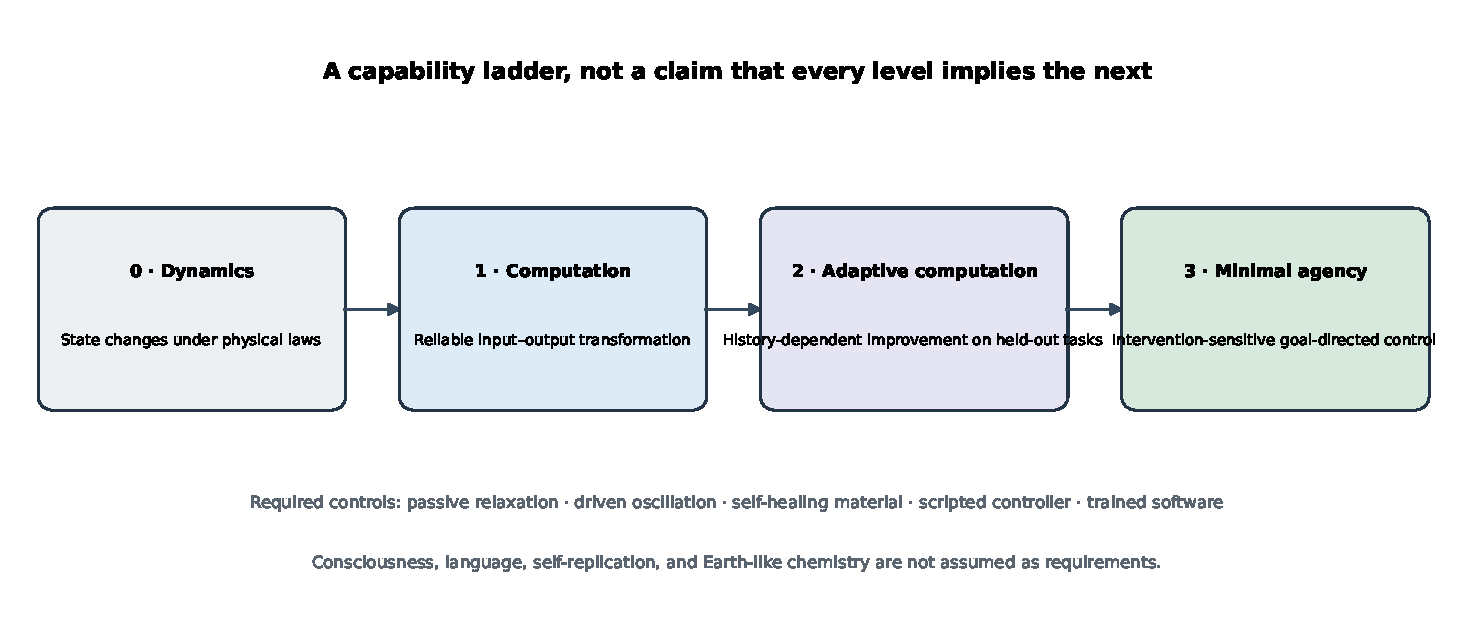
\includegraphics[width=0.98\linewidth]{fig2_capability_ladder.pdf}
\caption{A capability ladder from ordinary physical dynamics to a candidate minimal agency. Passing one level does not imply the next. In particular, a physical system can compute without learning, and can learn a task without possessing autonomous goals.}
\label{fig:ladder}
\end{figure}

This hierarchy prevents a common inferential error: equating complexity with intelligence. A crystal can encode a history in defect patterns; a driven oscillator can exhibit memory; a self-healing polymer can return towards a previous state; and a chemical reservoir can solve a prediction task. Each may be scientifically interesting without meeting the stronger criteria of learning, generalisation, and goal-directed control. Agency theories emphasise individuality, normativity, interactional asymmetry, and spatiotemporal continuity, but these concepts require careful operationalisation before they can serve as remote detection criteria \citep{Barandiaran2009}.

\subsection{Operational criteria}

For a candidate system with hidden state $x_t$, input or perturbation $u_t$, environmental conditions $e_t$, and observation $y_t$, write
\begin{align}
  x_{t+1} &= F_{\theta}(x_t,u_t,e_t,\xi_t), \\
  y_t &= G_{\theta}(x_t,e_t,\epsilon_t),
\end{align}
where $\xi_t$ and $\epsilon_t$ represent process and measurement noise, and $\theta$ includes unknown material parameters. The framework does not require that $F_\theta$ or $G_\theta$ be known in advance. Instead, it requires controlled interventions and comparison with plausible non-agent models.

We propose five dimensions:
\begin{enumerate}
  \item \textbf{Computational responsiveness ($C$).} Does the system implement a reproducible mapping between deliberately varied inputs and measured outputs? A useful baseline is mutual information $C=\MI(U_{t:t+\tau};Y_{t:t+\tau})$, evaluated under a declared input distribution and against passive and instrument-only controls.
  \item \textbf{Persistent memory ($M$).} Does information about earlier inputs improve prediction of future outputs after conditioning on the currently measured state, present input, and environmental variables? One candidate statistic is $M_k=\MI(Y_{t+1};U_{t-k:t-1}\mid Y_t,U_t,E_t)$. Hidden state, hysteresis, and sensor lag can produce apparent memory, so the measurement model must be challenged.
  \item \textbf{Adaptive learning ($L$).} Does interaction produce a persistent improvement in task performance on previously unseen conditions? Define $L=\E[J(\pi_{\mathrm{updated}},Z_{\mathrm{test}})-J(\pi_{\mathrm{fixed}},Z_{\mathrm{test}})]$, where $Z_{\mathrm{test}}$ is held out, $J$ is a pre-registered task score, and the comparison controls for drift and additional energy input.
  \item \textbf{Predictive control ($P$).} Does the system use information about future consequences to select actions that causally improve a pre-specified objective? Compare policies under interventions, for example $P=\E[J\mid\doop(\pi_{\mathrm{adaptive}})]-\E[J\mid\doop(\pi_{\mathrm{random}})]$.
  \item \textbf{Transfer and autonomy ($T,A$).} Does the system preserve useful performance under novel perturbations, and does the control loop continue without an external operator specifying every response? Transfer should be tested on distribution shifts, not merely on repeated instances of the training set.
\end{enumerate}

No single score should be treated as a universal intelligence meter. The vector $(C,M,L,P,T,A)$ is a structured profile, and the thresholds depend on the task, sensor, environmental scale, and null models. Consciousness, language, human-like reasoning, self-replication, and self-repair are not assumed to be necessary conditions. Self-maintenance may be relevant to autonomous agency, but the absence of replication does not by itself rule out intelligence.

\section{What nature has already demonstrated: computation without a brain}

\subsection{Chemical reaction networks as computational substrates}

The strongest empirical bridge between natural matter and non-biological computation is no longer purely hypothetical. Baltussen and colleagues demonstrated a chemical reservoir computer based on the formose reaction in a continuously stirred reactor. The self-organising reaction network performed nonlinear classification tasks, predicted dynamics of other systems, and forecast time series using measured chemical states and a trained linear readout \citep{Baltussen2024}. This is a direct demonstration of computational function in a chemical substrate. It is not evidence that the reaction network independently selected tasks, learned its own objective, or formed an autonomous agent; the experimental system had externally specified inputs and a trained readout.

This distinction is central. A reservoir can be computationally useful because its physical dynamics transform and retain information. The training algorithm may reside outside the reservoir. A future experiment that claims adaptation must therefore identify where learning occurs: in the substrate, in an external controller, in a human-designed readout, or in the interaction among them. The system boundary cannot be chosen after seeing the result.

\subsection{Physical reservoir computing}

Physical reservoir computing uses material dynamics rather than a fully simulated recurrent network. Candidate substrates include electronic, optical, mechanical, and other dynamical systems. The 2024 tutorial by Stepney lays out the key distinction between a physical system that merely evolves and one that performs a defined computation: there must be an input encoding, suitable internal state dynamics, a readout, and task-based characterisation \citep{Stepney2024}. The important implication for astrobiology is methodological. Computation can be physically implemented in many substrates, but task-specific computational performance does not establish open-ended intelligence.

\subsection{Autocatalysis and the origin-of-life boundary}

Autocatalytic networks provide a separate, potentially more consequential bridge. In RAF theory, a reaction set is reflexively autocatalytic and food-generated when each reaction is catalysed by elements in the set and the reactants can be generated from an environmental food set through the set's own reactions. Hordijk and Steel review the role of such networks in chemical organisation and origins-of-life theory, while cautioning that autocatalytic closure is not by itself a complete definition of life \citep{HordijkSteel2018}. RAF-like structure could supply persistence and self-production, but the existence of a catalytic loop does not demonstrate information-guided learning or goal-directed control.

The abiotic-to-prebiotic-to-biotic transition is itself difficult to reconstruct from snapshots. Barge and colleagues (2026) argue that planetary organic chemical evolution changes the meaning and visibility of biosignatures across time; a chemical state may sit along a continuum between abiotic, prebiotic, and biotic processes \citep{Barge2026}. That lesson applies directly to this paper: an unusual chemical organisation should not be labelled either life or intelligence solely from its material complexity.

\subsection{Planetary-scale organisation}

Frank, Grinspoon, and Walker proposed treating intelligence as a planetary-scale process, asking whether technological intelligence can be understood as a transition involving a planet's coupled systems rather than only an individual organism \citep{Frank2022}. Their framework is not a claim that planets are conscious or that non-living planets independently become intelligent. It does motivate multi-scale questions: can feedback among atmosphere, hydrosphere, lithosphere, biosphere, and technology generate system-level causal organisation? A planetary-scale system could be an adaptive collective without being a single centralised agent. This distinction matters for detecting distributed and post-biological systems.

\section{Three origin hypotheses and a two-axis taxonomy}

We consider three competing explanations for an observed non-biological candidate:
\begin{description}
  \item[$\HD$ (direct emergence):] natural processes produce a persistent, adaptive information-processing system without a preceding biological evolutionary lineage or a prior intelligence deliberately constructing it.
  \item[$\HC$ (constructed origin):] an earlier biological or non-biological intelligence deliberately designs or assembles the system, perhaps followed by autonomous persistence or further evolution.
  \item[$\HN$ (natural non-agent):] an abiotic process produces a complex or apparently responsive system that does not meet the functional criteria for adaptive intelligence.
\end{description}

A fourth pathway, biological evolution into unfamiliar non-terrestrial life, is not a subcase of $\HD$. It belongs on the biological side of the causal-origin distinction even if its substrate differs radically from Earth life. Likewise, a constructed system could eventually become self-modifying and autonomous; its present capabilities do not erase its constructed ancestry.

\begin{figure}[H]
\centering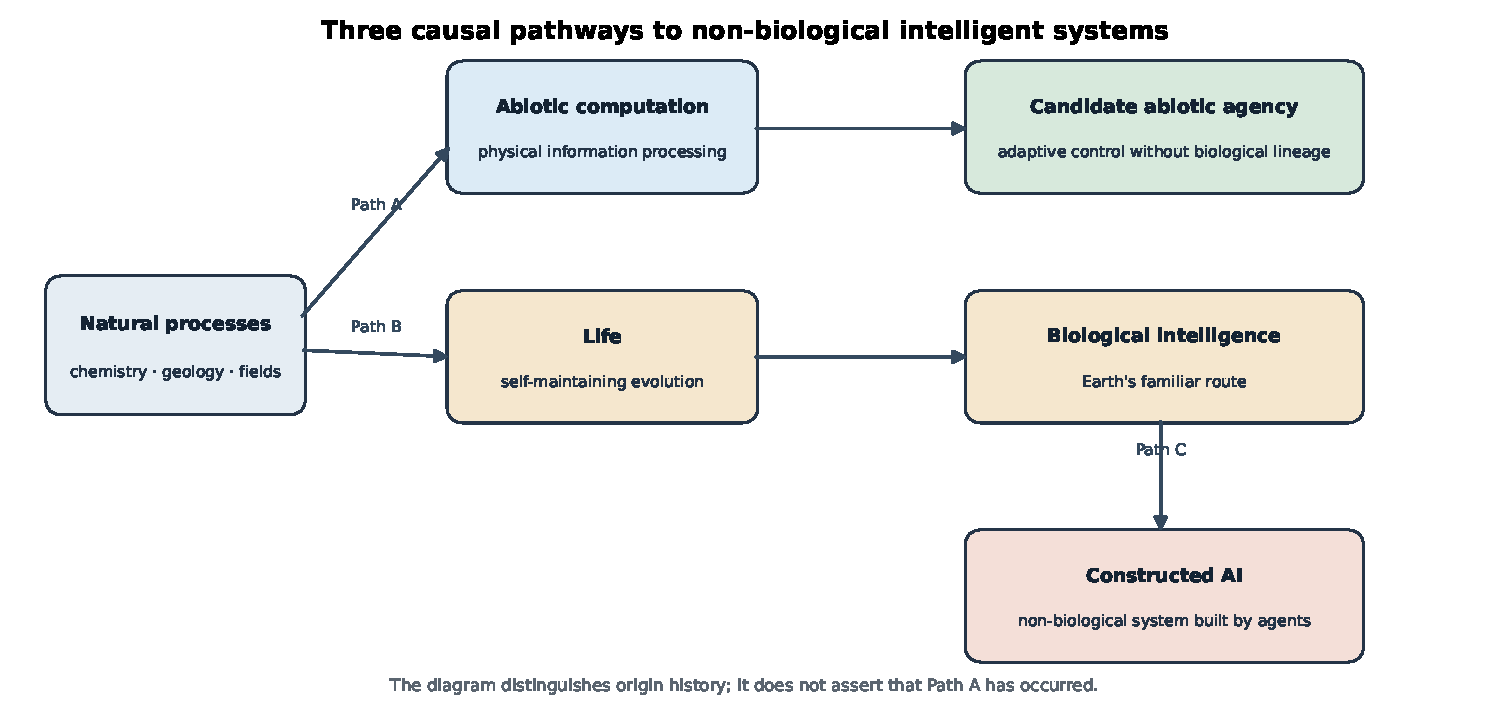
\includegraphics[width=0.98\linewidth]{fig1_pathways.pdf}
\caption{Three paths to non-biological systems with intelligence-like properties. Path A is the hypothesis of direct abiotic emergence. Path B is the familiar Earth-like biological route. Path C is intelligence-mediated construction. Arrows denote hypothesised causal histories, not established universal sequences.}
\label{fig:pathways}
\end{figure}

The taxonomy has two axes: \emph{implementation substrate} and \emph{causal origin}. These must not be collapsed. A naturally emerged system could use chemistry, mineral networks, plasma, optical fields, or an unfamiliar medium; a constructed system could use those same substrates. Consequently, no material signature is intrinsically a proof of artificiality, and no unusual substrate is proof of abiotic emergence.

\begin{table}[H]
\centering\small
\caption{Candidate substrate classes and their evidential status.}
\label{tab:substrates}
\begin{tabularx}{\linewidth}{p{0.20\linewidth}p{0.36\linewidth}X}
\toprule
Substrate & Demonstrated or plausible physical role & What is not yet demonstrated \\
\midrule
Chemical reaction networks & Experimentally demonstrated reservoir computation in the formose reaction; nonlinear classification and time-series prediction \citep{Baltussen2024}. & Autonomous task selection, internally generated objectives, open-ended learning, or abiotic intelligence. \\
Mineral / catalytic networks & Mineral surfaces and inorganic catalysts are relevant to prebiotic chemistry; autocatalytic organisation has a formal graph-theoretic description \citep{HordijkSteel2018}. & Persistent adaptive control or intelligent agency in a naturally occurring mineral network. \\
Electronic / optical / mechanical media & Laboratory physical reservoirs can exploit material dynamics for computing \citep{Stepney2024}. & Independent natural emergence of a self-maintaining intelligent agent in these media. \\
Plasma and atmospheric systems & Nonlinear self-organisation and long-lived structures motivate candidate physical models. & Reliable memory, learning, prediction, and goal-directed control; no evidence of plasma intelligence. \\
Planetary coupled systems & Planetary-scale feedback and technosphere-biosphere coupling motivate system-level analysis \citep{Frank2022}. & A planet-wide autonomous agent or intelligence independent of biology. \\
\bottomrule
\end{tabularx}
\end{table}

The plasma and planetary cases are included as research directions, not as evidence of intelligence. In particular, self-organisation, filamentation, pattern formation, or persistence must not be anthropomorphised. A natural phenomenon should be promoted to a computational or agency hypothesis only after controlled tests distinguish it from ordinary dissipative dynamics.

\section{The origin-identifiability problem}

\subsection{Functional evidence and provenance evidence}

Let the observation record be partitioned into four channels:
\begin{equation}
  D=(D_F,D_T,D_P,D_C),
\end{equation}
where $D_F$ contains functional measurements (computation, memory, learning, transfer, control); $D_T$ contains thermodynamic and energy-flow measurements; $D_P$ contains provenance evidence (manufacturing traces, repeated design motifs, assembly signatures, or historical records); and $D_C$ contains environmental and contextual evidence (geology, orbital setting, age, surrounding chemistry, and possible sources of energy or feedstock).

The posterior probability of an origin hypothesis is
\begin{equation}
  P(H_i\mid D)=\frac{P(D\mid H_i)P(H_i)}{\sum_j P(D\mid H_j)P(H_j)},
  \label{eq:bayes}
\end{equation}
with nuisance parameters integrated rather than fixed at convenient values:
\begin{equation}
  P(D\mid H_i)=\int P(D\mid H_i,\theta_i)\,p(\theta_i\mid H_i)\,d\theta_i.
\end{equation}
A credible comparison therefore requires explicit model families, prior sensitivity analysis, and null models broad enough to include natural complexity and engineered decoys.

\subsection{Proposition: functional equivalence prevents origin inference}

\textbf{Proposition 1 (functional non-identifiability).} Suppose that the direct-emergence and constructed-origin hypotheses induce identical likelihoods for every functional observation in the available record:
\begin{equation}
  P(D_F\mid\HD)=P(D_F\mid\HC).
  \label{eq:equal}
\end{equation}
Then the Bayes factor based on functional evidence alone is
\begin{equation}
  BF_{D,C}(D_F)=\frac{P(D_F\mid\HD)}{P(D_F\mid\HC)}=1,
\end{equation}
and posterior odds equal prior odds:
\begin{equation}
  \frac{P(\HD\mid D_F)}{P(\HC\mid D_F)}=
  \frac{P(\HD)}{P(\HC)}.
\end{equation}
\emph{Proof.} Substitute Eq.~\ref{eq:equal} into Bayes' rule; the common likelihood cancels. The result follows directly. \hfill$\square$

The proposition is simple but consequential. If a naturally emerged agent and a constructed agent can both learn, predict, repair, self-modify, and act autonomously, observing those behaviours does not by itself reveal which history occurred. A classifier cannot recover causal history from a feature set whose probability distributions are identical under the competing histories. The relevant information must come from provenance, temporal records, environmental context, or some other channel whose distributions differ.

A softer version uses the Kullback--Leibler divergence. If $\KL(P(D_F\mid\HD)\Vert P(D_F\mid\HC))$ is small, functional evidence is weak for origin classification even if it is strong for identifying a system as an adaptive information processor. Conversely, a large divergence in a reliably measured provenance channel could increase the Bayes factor, but the model for that channel must itself be tested against natural mimics and preservation bias.

\subsection{Why provenance is difficult}

Provenance is not a simple manufactured-versus-natural checkbox. A constructed entity may be old enough for its construction marks to erode, be self-replicating, or use local materials and distributed assembly. A naturally emerged system may develop modular structures, repeated motifs, or highly regular geometries. Natural selection can generate design-like organisation; geology can generate regularity; and human artefacts can become chemically and structurally altered. The inference is historical and abductive, not a visual classification exercise.

The search for technosignatures already distinguishes communicative signals from artefacts, active technologies from derelict ones, and model-based searches from anomaly searches. Wright's overview emphasises both the breadth of technosignatures and the need to state the assumptions behind observational strategies \citep{Wright2021}. Our framework extends that caution: evidence for an artificial-looking object, a non-biological substrate, or an intelligent-looking signal should not be conflated with evidence for the direct natural emergence hypothesis.

\section{A reproducible synthetic identifiability demonstration}

To make Proposition 1 concrete, we implemented a small generative model. It is deliberately pedagogical and uses no astronomical, laboratory, or biological observations. Three classes are generated: direct abiotic emergence ($\HD$), constructed non-biological intelligence ($\HC$), and a non-intelligent abiotic decoy ($\HN$). A functional score $F$, a provenance score $P$, and a response-transfer score $R$ are sampled from Gaussian distributions with clipped support on $[0,1]$. The means and standard deviations are listed in the accompanying source code and output file.

The defining assumption is that the functional score has the same stipulated distribution for $\HD$ and $\HC$. This encodes functional equivalence by construction. The provenance score is stipulated to differ between the two origin classes. It is not asserted that real provenance evidence always has these distributions or is detectable remotely.

\begin{figure}[H]
\centering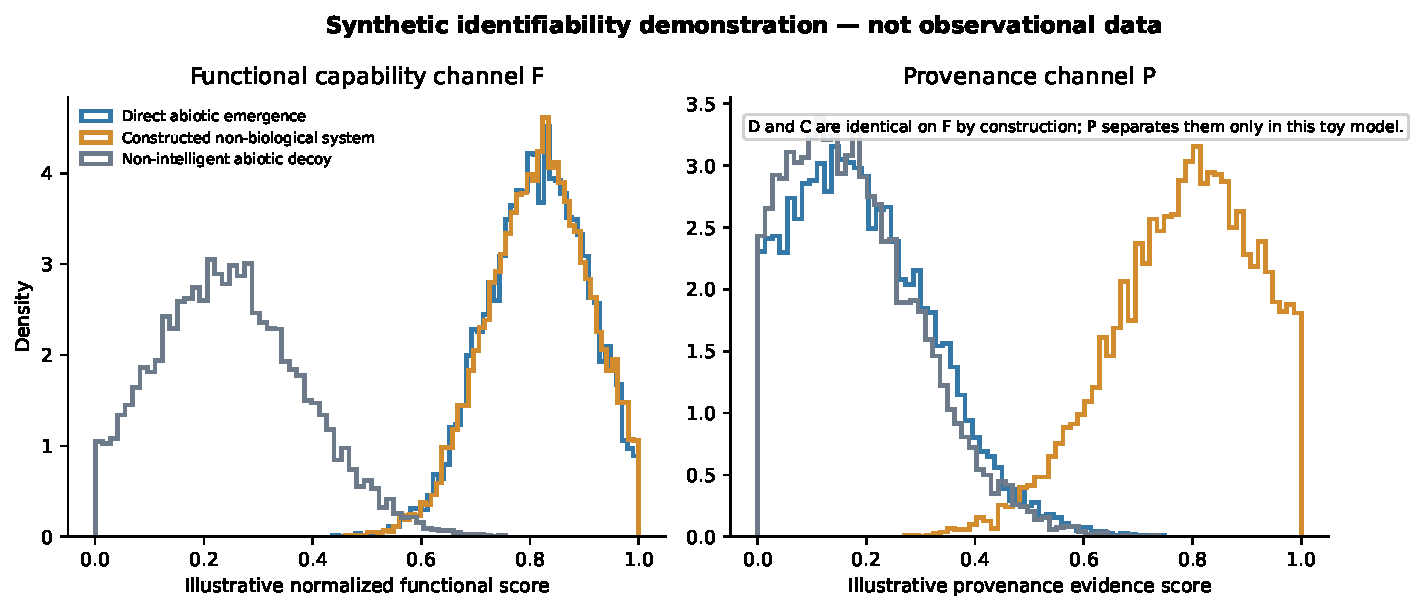
\includegraphics[width=0.98\linewidth]{fig3_identifiability.pdf}
\caption{Synthetic distributions used to illustrate identifiability. The two intelligence-origin classes share the same functional-score distribution by construction. The provenance channel differs in this toy model. These curves are assumed distributions, not empirical signatures.}
\label{fig:synthetic}
\end{figure}

With 10,000 Monte Carlo samples per class and fixed seed 20261030, a Gaussian likelihood classifier distinguished direct emergence from construction with 0.500 accuracy using $F$ alone. Adding the assumed provenance feature increased accuracy to 0.982. In a separate illustrative threshold test, pooling $\HD$ and $\HC$ as functional-intelligence candidates and comparing them with $\HN$ produced sensitivity 0.9985 and specificity 0.9764 under the selected synthetic score distributions.

\begin{table}[H]
\centering\small
\caption{Synthetic demonstration results. These figures are generated from hand-specified class distributions and must not be interpreted as expected performance on exoplanets or real materials.}
\label{tab:results}
\begin{tabularx}{0.99\linewidth}{>{\raggedright\arraybackslash}X>{\raggedright\arraybackslash}X>{\raggedright\arraybackslash}X}
\toprule
Task & Features used & Accuracy / estimate \\
\midrule
Direct emergence vs. construction & Functional score only ($F$) & 0.500 \\
Direct emergence vs. construction & Function plus provenance ($F,P$) & 0.982 \\
Functional-intelligence candidate vs. non-agent decoy & Threshold on $F$ & Sensitivity 0.9985; specificity 0.9764 \\
\bottomrule
\end{tabularx}
\end{table}

The large improvement is not a scientific prediction. It demonstrates only that a provenance channel can resolve an ambiguity when the toy model stipulates different provenance distributions. In reality, provenance may be absent, erased, inaccessible, or mimicked. The central result is not the 0.982 number; it is the 0.500 result under functional equivalence and the explicit dependence of origin inference on evidence beyond functional behaviour. The full script, fixed seed, parameterisation, and machine-readable output are included with the release.

\section{Thermodynamics and the physical costs of computation}

A candidate intelligent system must obey the physical constraints of its substrate. For a system exchanging matter and energy with an environment, an energy budget and entropy balance can constrain whether proposed memory, control, and learning mechanisms are physically plausible. At the minimum, repeated information processing requires a physical state space and a mechanism for preserving, transforming, and sometimes erasing information.

Landauer's principle gives a lower bound for an ideal logically irreversible erasure of one bit at temperature $T$:
\begin{equation}
  Q_{\min}=k_{\mathrm B}T\ln 2.
  \label{eq:landauer}
\end{equation}
This is not a universal energy cost for every computation, nor does it imply that any observed heat source identifies intelligence. Reversible computation, finite-time control, correlations with the environment, and error correction complicate practical energetic bounds. The principle is useful because information processing is physically embodied, not because it supplies an intelligence-specific biosignature \citep{Landauer1961,Wimsatt2021}.

For a candidate system, useful measurements include energy throughput, temperature, gradients, relaxation times, dissipation, environmental coupling, and the response of memory-like states to controlled perturbations. A system that appears to maintain a complex internal state may simply be driven by an external power source. A system that reduces local entropy may export entropy to its surroundings. Thermodynamic observations must therefore be embedded in a defined control volume and energy budget.

A particularly exotic question is whether a natural system can exploit gradients to support computation and adaptive control without a biological metabolism. The chemical reservoir result makes the computational part experimentally plausible in a limited sense. Whether a corresponding substrate can autonomously discover useful representations, learn new environmental contingencies, and maintain its own organisation remains open.

\section{Candidate substrates and environments}

\subsection{Chemical and geochemical networks}

Chemical networks are the most experimentally tractable starting point because their reaction states can be manipulated and measured. A programme could combine formose-like reservoirs, metal-ion catalysis, mineral surfaces, and flow-driven reactors. Inputs should include novel temporal sequences, perturbations to feedstock concentrations, removal or addition of candidate catalysts, and controlled changes in energy gradients. The critical test is not whether the system produces a complex output, but whether it updates its internal dynamics in a way that improves performance on unseen task instances after the external trainer is removed.

Geochemical systems offer long-lived, spatially extended reaction networks. Hydrothermal gradients, mineral interfaces, and redox couples are relevant as natural energy and matter sources. RAF theory offers a route to quantify catalytic closure, but closure must be separated from learning and agency. A mineral network that amplifies a reaction is not thereby an agent.

\subsection{Plasma and electromagnetic systems}

Plasma is attractive as a speculative substrate because it supports nonlinear collective dynamics, electromagnetic coupling, and self-organised structures. But the evidential gap is large. A long-lived plasma structure or filament can arise from ordinary field dynamics without storing task-relevant information, learning from interventions, or selecting actions. A rigorous experiment would need to demonstrate controlled input-output mappings, state-dependent memory, held-out task improvement, and causal control, while accounting for external field sources and measurement artefacts. We found no empirical demonstration of plasma intelligence; this paper treats it strictly as a candidate modelling domain.

\subsection{Atmospheric and planetary systems}

Atmospheres, oceans, crusts, magnetic fields, and surface chemistry form coupled, multiscale systems with feedback loops. A planetary system might exhibit robust regulation or collective adaptation without containing a single localised controller. The planetary-intelligence framing of Frank et al. encourages analysis at that scale, but the transition from feedback-rich planetary dynamics to intelligence remains unproved \citep{Frank2022}. A planetary system might be computationally rich without being an agent, just as climate dynamics encode and transform information without being intelligent.

\subsection{Artificial and post-biological substrates}

If a civilisation constructs non-biological intelligence, its descendants may persist after the civilisation disappears. A post-biological entity could use local materials, alter its structure, and adapt to an environment. It may no longer preserve easily recognisable artefacts of its creators. Conversely, a naturally emerged abiotic agent could acquire persistent structure and leave records that look designed. This makes temporal and environmental evidence central to origin attribution.

\section{A staged detection framework}

We propose that candidate evaluation proceed in four stages rather than jumping directly from anomaly to origin claim.

\begin{figure}[H]
\centering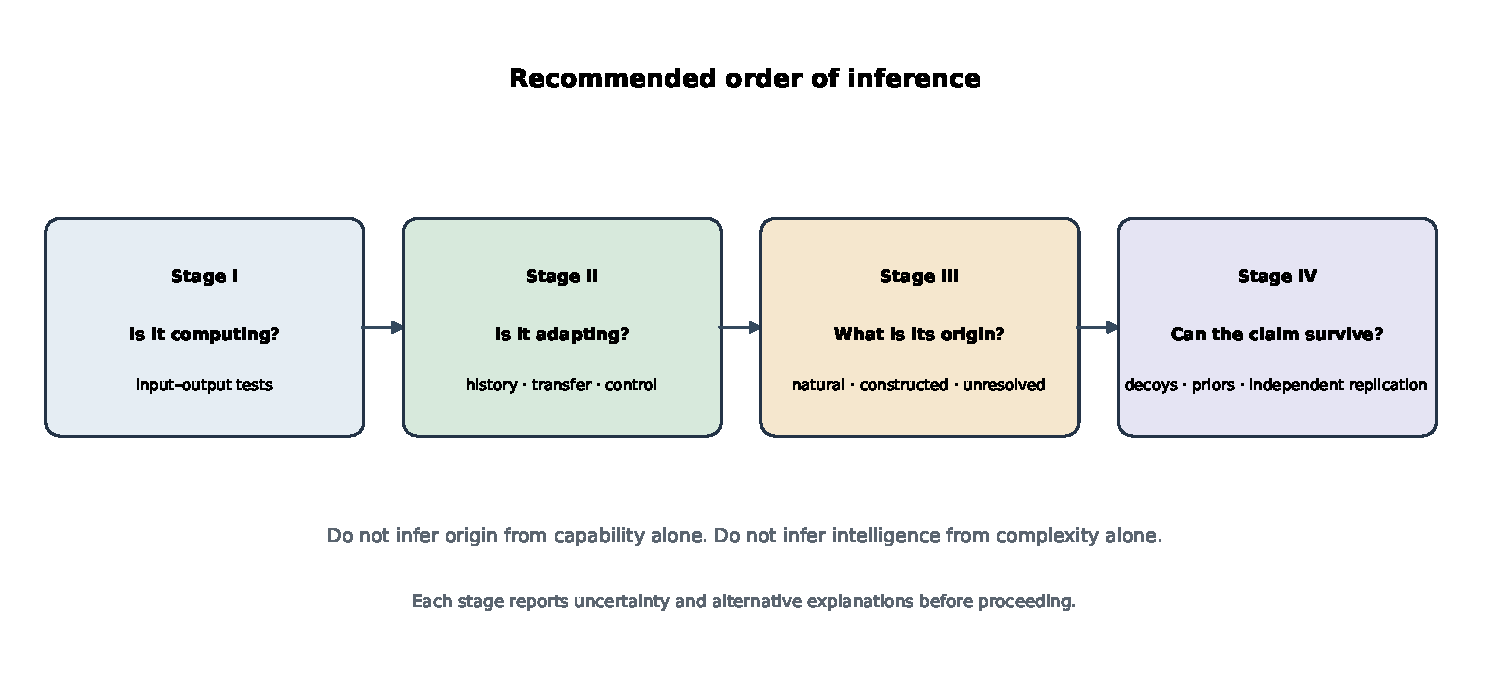
\includegraphics[width=0.98\linewidth]{fig4_inference_pipeline.pdf}
\caption{Recommended staged inference: establish task-defined computation, test adaptation and agency, assess causal origin, and then stress-test the full claim against decoys, prior sensitivity, and independent replication.}
\label{fig:pipeline}
\end{figure}

\subsection{Stage I: establish computation}

Specify the physical boundary of the candidate, the input and output channels, the task distribution, the sensor model, and a set of null systems. Use controlled perturbations where possible. The null family should include passive relaxation, driven oscillators, hysteretic materials, self-healing systems, deterministic chaos, scripted controllers, and instrument artefacts. A system is not a computer merely because a sufficiently flexible algorithm can fit its observed time series; the input-output relation must be stable and counterfactually testable.

\subsection{Stage II: establish adaptation and minimal agency}

Use sequential tasks that separate memory, learning, and transfer. A suitable protocol contains: (i) baseline characterisation; (ii) randomised training perturbations; (iii) a washout or reset phase; (iv) novel held-out perturbations; (v) adversarial decoys engineered to reproduce one or more response features; and (vi) independent replication with blinded analysis. The system should show improvement attributable to its own updated state or policy, not merely to external recalibration. To claim agency, the experiment should identify a system boundary and show that interventions on its action channel causally affect a maintained objective.

The earlier repository preprint, \emph{Interrogating Alien Life}, proposes an adaptive-probing benchmark for repair-like dynamics and synthetic abiotic decoys. The present paper addresses a different question: even if an entity passes a functional test, what evidence could distinguish a naturally emerged origin from construction? Repair-like behaviour can be one feature within Stage II, but is neither a definition of intelligence nor a provenance marker.

\subsection{Stage III: infer origin}

After functional capability is established, compare $\HD$, $\HC$, and $\HN$ using the full observation record. Candidate provenance evidence may include manufacturing processes, modular interfaces, non-random assembly constraints, material refinement, records of staged construction, orbital or geological placement, and long-baseline changes inconsistent with known environmental processes. Each item requires a natural mimic model. Repeated geometric regularity alone is weak evidence; a convincing case would require multiple independent channels with quantified dependence and preservation uncertainties.

\subsection{Stage IV: stress-test and report uncertainty}

Use Bayesian model comparison with prior sensitivity, cross-validation where data volume permits, and out-of-distribution null families. Report the probability of alternative explanations, not only the most likely label. Null detections and failed measurements should also be retained. Recent astrobiology literature highlights false negatives as well as false positives in life searches, including effects of abundance, activity, preservation, location, and instrument limitations \citep{tenKate2026}. A search for unfamiliar intelligence will face analogous blind spots: an entity may be dormant, low-power, distributed, or simply outside the observing cadence and spectral bands.

Any claim of an extraterrestrial-intelligence detection must also follow community verification and communication protocols. The International Academy of Astronautics published an updated SETI Declaration of Principles on 1 June 2026, including guidance for candidate handling, verification, public communication, data access, and post-detection governance \citep{IAA2026}. An abiotic-origin claim would require an additional layer of careful scientific qualification; a functional anomaly alone is not a confirmed detection.

\section{Predictions, falsifiers, and experimental programme}

The framework yields testable expectations rather than a claim of discovery.
\begin{enumerate}
  \item \textbf{Computation without agency should be commoner than intelligence.} Many nonlinear physical systems should pass narrow computational benchmarks but fail tests of autonomous learning, goal maintenance, and transfer. This prediction is testable in laboratory reservoirs and materials.
  \item \textbf{Functional performance will not generally identify provenance.} If direct-emergence and constructed systems converge on similar functional architectures, then origin classification from behaviour-only data will be weak. This can be tested in deliberately constructed laboratory benchmarks where origin labels are known and functional behaviour is matched.
  \item \textbf{Independent provenance evidence should add information only when calibrated.} Material or historical features may improve origin inference, but the gain should collapse under natural-mimic controls, preservation uncertainty, or model misspecification. This is an explicit falsifier of overconfident artificiality classification.
  \item \textbf{Novel-context transfer is more diagnostic than repeated recovery.} A system that succeeds only on repeated training perturbations may be a specialised relaxor or controller. Performance on new contexts, under blinded protocols, provides a stronger test of adaptive computation.
  \item \textbf{Thermodynamic consistency is necessary but not sufficient.} Candidate information-processing mechanisms must be energetically and entropically plausible, but a physically plausible energy budget is not unique to intelligent systems.
\end{enumerate}

A first experimental sequence should use chemical reservoir platforms because their reaction states, input flows, and readouts are already measurable. The next step would be to move beyond externally trained readouts: define a task with a changing environment, allow the reaction network to alter its own state or reaction pathways through local feedback, and test whether it improves on unseen contingencies without a supervising controller. A second sequence could use mineral-catalytic networks in geochemical microfluidic cells. Plasma and planetary-scale models should follow only after the operational tests are made tractable in controlled systems.

The key experimental controls are system boundary, instrument drift, external forcing, hidden controllers, readout training, selection bias, and task leakage. Experiments should preregister task families and failure criteria, use multiple seeds or independent physical replicates, include adversarial decoys, and release raw measurements and analysis code. A positive result would establish a capability under defined conditions; it would not, by itself, establish that the same phenomenon occurs naturally on an exoplanet.

\section{Limitations and epistemic status}

The proposal has important limitations. Intelligence is not a single universally accepted physical observable. The operational criteria here intentionally target functional capacities and do not settle questions about consciousness, subjective experience, semantics, or moral status. Measurement channels may fail to transfer across substrates. A sufficiently flexible external controller can make a passive substrate appear adaptive if the system boundary is drawn incorrectly. Natural and engineered systems can converge in organisation, and provenance traces may be lost over geological timescales.

The synthetic demonstration is especially limited: its distributions are selected by the authors to express a known identifiability scenario. Its classification accuracy says nothing about real-world detectability. It is a unit test for the inference logic, not a benchmark of alien-intelligence detection. The literature search was targeted rather than systematic, and no claim of priority or complete novelty is made. The principal contribution is an integration of physical computation, operational agency tests, and origin identifiability into one disciplined research question.

The paper also does not claim that biological evolution is unnecessary for all forms of intelligence. It asks whether necessity has been established. At present, there is no evidence that a naturally occurring non-biological system has independently crossed the proposed capability ladder to intelligence. The chemical reservoir result demonstrates an intermediate computational capability, not the final transition.

\section{Conclusion}

Earth's route from natural processes through biological intelligence to engineered AI is one observed path. It is not, by itself, proof that biology is a universal bottleneck. Contemporary physical computing and chemical reservoir experiments show that useful computation can be implemented in non-neural, non-digital material substrates. Autocatalytic network theory, nonequilibrium thermodynamics, causal emergence, and planetary-scale systems provide further tools for asking how complex organisation persists and interacts with its environment. Yet computation is not agency, and agency is not automatically intelligence.

The second question is as important as the first. If a non-biological intelligent system were detected, its functional capabilities would not reveal whether it emerged directly from natural processes or was constructed by an earlier intelligence. Proposition 1 formalises this limitation: when functional likelihoods coincide, functional data cannot update origin odds. Evidence about origin must come from additional, independently calibrated provenance, contextual, thermodynamic, or historical channels.

The most useful next step is therefore not to declare that plasma, minerals, or planets are intelligent. It is to develop experimental systems in which computation, learning, transfer, and control can be separately measured; to challenge them with strong natural decoys; and to design provenance tests that remain valid under natural mimicry and information loss. The biological bottleneck may be real, or it may be an artefact of the only example currently known. Distinguishing those possibilities is an empirical research programme.

\section*{Research-process credit and disclosure}
This manuscript was prepared with AI-assisted literature discovery, synthesis, drafting support, and code generation. The named human author is responsible for the final selection of claims, interpretation, source checking, and release. AI assistance is not represented as a human co-author. The synthetic code and outputs are reproducible, and no empirical biological, astronomical, or extraterrestrial datasets were used.

\begin{thebibliography}{99}
\bibitem{Baltussen2024} M. G. Baltussen, T. J. de Jong, Q. Duez, W. E. Robinson, and W. T. S. Huck, ``Chemical reservoir computation in a self-organizing reaction network,'' \emph{Nature}, vol. 631, pp. 549--555, 2024. doi: \href{https://doi.org/10.1038/s41586-024-07567-x}{10.1038/s41586-024-07567-x}.
\bibitem{Stepney2024} S. Stepney, ``Physical reservoir computing: a tutorial,'' \emph{Natural Computing}, vol. 23, pp. 665--685, 2024. doi: \href{https://doi.org/10.1007/s11047-024-09997-y}{10.1007/s11047-024-09997-y}.
\bibitem{HordijkSteel2018} W. Hordijk and M. Steel, ``Autocatalytic networks at the basis of life's origin and organization,'' \emph{Life}, vol. 8, no. 4, article 62, 2018. doi: \href{https://doi.org/10.3390/life8040062}{10.3390/life8040062}.
\bibitem{Frank2022} A. Frank, D. Grinspoon, and S. Walker, ``Intelligence as a planetary scale process,'' \emph{International Journal of Astrobiology}, vol. 21, no. 2, pp. 47--61, 2022. doi: \href{https://doi.org/10.1017/S147355042100029X}{10.1017/S147355042100029X}.
\bibitem{Graham2026} H. V. Graham, ``Agnostic biosignatures: expanding the search for life in the Solar System,'' \emph{Annual Review of Earth and Planetary Sciences}, vol. 54, pp. 585--604, 2026. doi: \href{https://doi.org/10.1146/annurev-earth-040722-101044}{10.1146/annurev-earth-040722-101044}.
\bibitem{Barge2026} L. M. Barge, J. L. Eigenbrode, G. Fournier, and B. Theiling, ``Emergence of biosignatures on Earth and implications for life detection,'' \emph{Proceedings of the National Academy of Sciences}, vol. 123, no. 33, e2520594123, 2026. doi: \href{https://doi.org/10.1073/pnas.2520594123}{10.1073/pnas.2520594123}.
\bibitem{Barandiaran2009} X. E. Barandiaran, E. Di Paolo, and M. Rohde, ``Defining agency: individuality, normativity, asymmetry, and spatio-temporality in action,'' \emph{Adaptive Behavior}, vol. 17, no. 5, pp. 367--386, 2009. doi: \href{https://doi.org/10.1177/1059712309343819}{10.1177/1059712309343819}.
\bibitem{Landauer1961} R. Landauer, ``Irreversibility and heat generation in the computing process,'' \emph{IBM Journal of Research and Development}, vol. 5, no. 3, pp. 183--191, 1961. doi: \href{https://doi.org/10.1147/rd.53.0183}{10.1147/rd.53.0183}.
\bibitem{Wimsatt2021} G. W. Wimsatt, A. B. Boyd, P. M. Riechers, and J. P. Crutchfield, ``Refining Landauer's stack: balancing error and dissipation when erasing information,'' \emph{Journal of Statistical Physics}, vol. 183, article 16, 2021. doi: \href{https://doi.org/10.1007/s10955-021-02733-1}{10.1007/s10955-021-02733-1}.
\bibitem{Neveu2018} M. Neveu, L. E. Hays, M. A. Voytek, M. H. New, and M. D. Schulte, ``The ladder of life detection,'' \emph{Astrobiology}, vol. 18, no. 11, pp. 1375--1402, 2018. doi: \href{https://doi.org/10.1089/ast.2017.1773}{10.1089/ast.2017.1773}.
\bibitem{Cleaves2023} H. J. Cleaves et al., ``A robust, agnostic molecular biosignature based on machine learning,'' \emph{Proceedings of the National Academy of Sciences}, vol. 120, no. 41, e2307149120, 2023. doi: \href{https://doi.org/10.1073/pnas.2307149120}{10.1073/pnas.2307149120}.
\bibitem{tenKate2026} I. L. ten Kate et al., ``False negatives in the search for extraterrestrial life,'' \emph{Nature Astronomy}, vol. 10, pp. 624--629, 2026. doi: \href{https://doi.org/10.1038/s41550-026-02863-0}{10.1038/s41550-026-02863-0}.
\bibitem{Wright2021} J. T. Wright, ``Strategies and advice for the search for extraterrestrial intelligence,'' \emph{Acta Astronautica}, vol. 188, pp. 203--214, 2021. doi: \href{https://doi.org/10.1016/j.actaastro.2021.07.021}{10.1016/j.actaastro.2021.07.021}.
\bibitem{IAA2026} International Academy of Astronautics, SETI Committee, ``Declaration of Principles Concerning the Conduct of the Search for Extraterrestrial Intelligence (2026 Update),'' 1 June 2026. Available: \url{https://iaa-seti-committee.github.io/}.
\bibitem{PriorAlien} D. Debnath, ``Interrogating Alien Life: Adversarially Trained Reinforcement Learning for Substrate-Agnostic Detection of Self-Repair Dynamics,'' research preprint, 17 October 2026. \url{https://github.com/Devanik21/The-Invention-Archive}.
\end{thebibliography}

\end{document}
